\documentclass[a4paper, 12pt]{article}
\usepackage{titling}
\usepackage{array}
\usepackage{booktabs}
\usepackage{enumitem}
\usepackage{graphicx}
\usepackage{hyperref}
\usepackage{amssymb}
%\usepackage{mathtools}
\usepackage{listings}
\usepackage{amsmath}
\usepackage{color} %red, green, blue, yellow, cyan, magenta, black, white
\setlength{\heavyrulewidth}{1.5pt}
\setlength{\abovetopsep}{4pt}
\setlength{\parindent}{0pt}
\graphicspath{{.}}
\usepackage{float}
\usepackage[margin=1in]{geometry}
\definecolor{mygreen}{RGB}{28,172,0} % color values Red, Green, Blue
\definecolor{mylilas}{RGB}{170,55,241}
% Must be after geometry
\usepackage{fancyhdr}
\pagestyle{fancy}
\fancyhf{}
\rhead{NN Homework 5}
\lhead{P.Lukin, E. Ovchinnikova}
\cfoot{\thepage}

\setlength{\droptitle}{-5em}

\title{Neural Networks  \\
				- Homework 5 -}
\author{Petr Lukin, Evgeniya Ovchinnikova}
\date{Lecture date: 31 October 2016}

\begin{document}

%-------------------------------------------------------------------------------
\lstset{language=Matlab,%
    %basicstyle=\color{red},
    breaklines=true,%
    morekeywords={matlab2tikz},
    keywordstyle=\color{blue},%
    morekeywords=[2]{1}, keywordstyle=[2]{\color{black}},
    identifierstyle=\color{black},%
    stringstyle=\color{mylilas},
    commentstyle=\color{mygreen},%
    showstringspaces=false,%without this there will be a symbol in the places where there is a space
    numbers=left,%
    numberstyle={\tiny \color{black}},% size of the numbers
    numbersep=9pt, % this defines how far the numbers are from the text
    emph=[1]{break},emphstyle=[1]\color{red}, %some words to emphasise
    %emph=[2]{word1,word2}, emphstyle=[2]{style},
}

%-------------------------------------------------------------------------------

\maketitle

\section{Mind map}

\begin{figure}[h]
  \centering
  \caption{Mind map. Chapter 3 (first part) from Haykin’s book. A zoomed version is attached as Single-Layer
  Perceptrons.png \label{fig:SingleLayer}}
  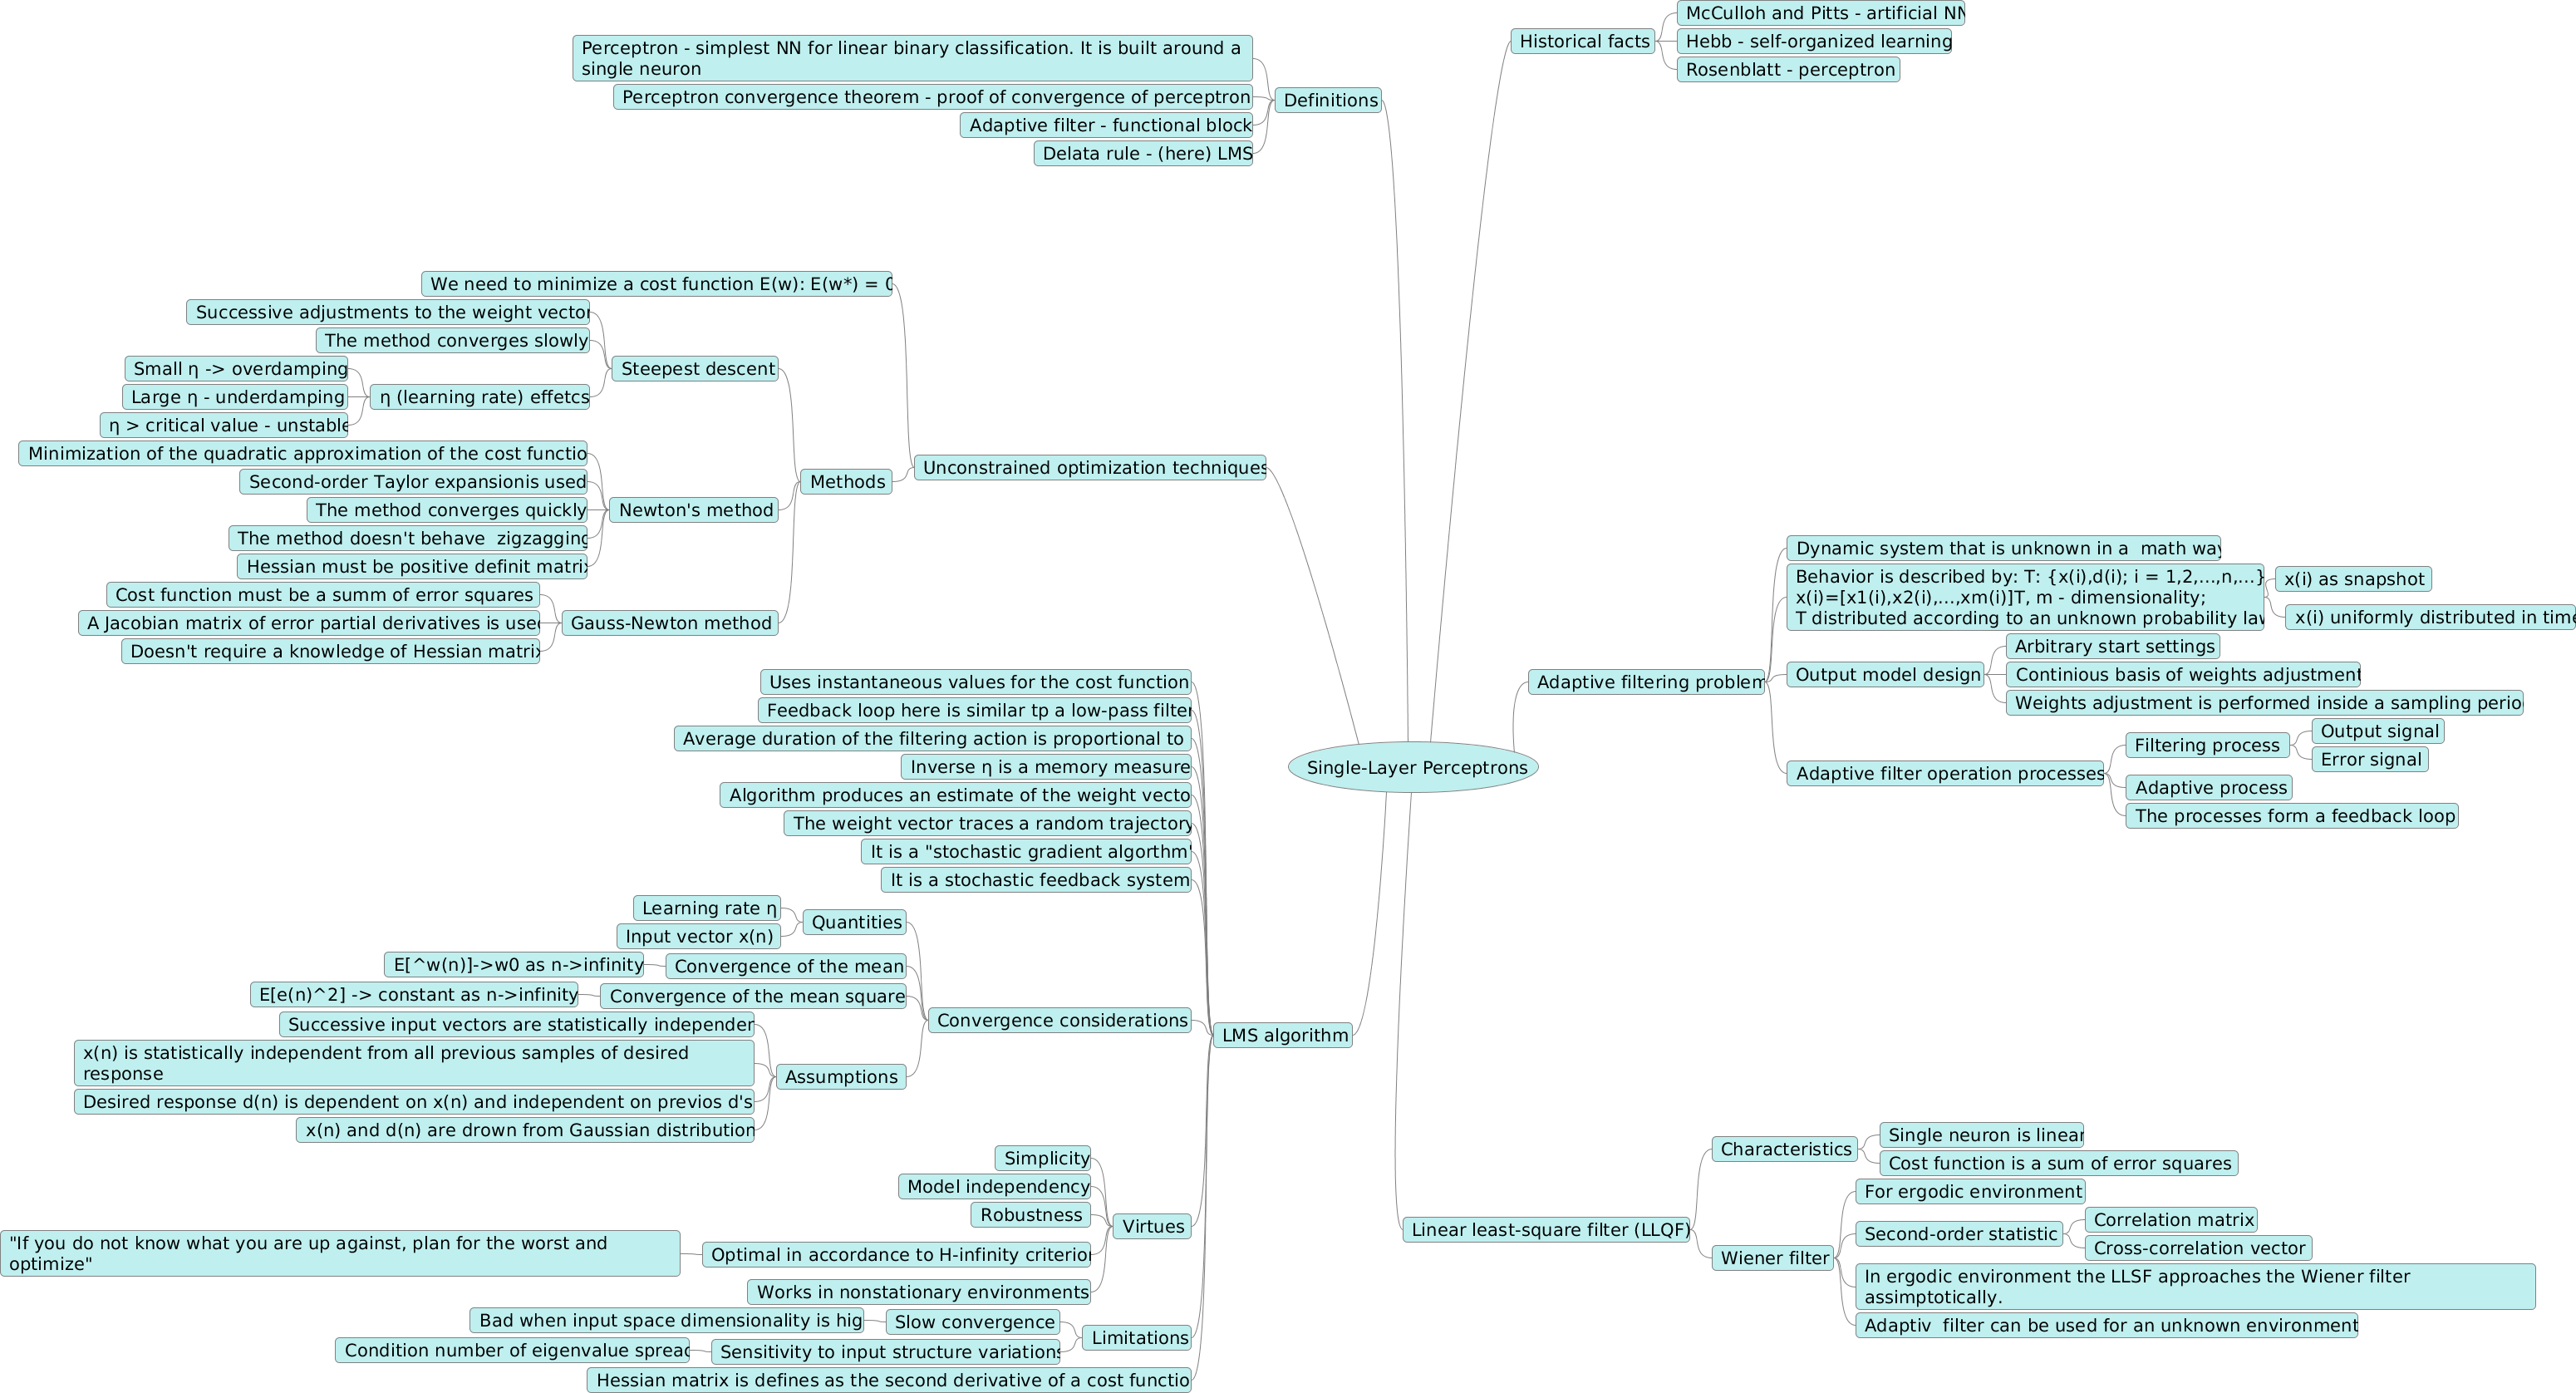
\includegraphics[width=1.0\textwidth]{Single-LayerPerceptrons}
\end{figure}

\section{Exercises}

\subsection{Exercise 3.1}
Explore the method of steepest descent involving a single weight w by considering the following cost function:\\

$\varepsilon(w) = \frac{1}{2} \sigma^2 - r_{xd}w + \frac{1}{2}r_x w^2$,\\

where $\sigma^2, r_{xd}$ and $r_x$ are constants.\\

Solution:\\

The steepest descent algorithm is describes as following:\\

$w(n+1) = w(n) - \eta g(n)$,\\
$\Delta w = -\eta g(n)$,\\

where $\eta$ is a learning rate that is a positive constant and $g(n)$ is a gradient vector evaluated in w(n) point:\\

$g(n) = \nabla \varepsilon(w) = [\frac{\partial \varepsilon}{\partial w_1}, \frac{\partial \varepsilon}{\partial w_2}, ... , \frac{\partial \varepsilon}{\partial w_m}]^T$, \\

where m is dimensionality of the input space.\\

$\varepsilon(w(n + 1)) \simeq \varepsilon(w(n)) - \eta ||g(n)||^2$\\

Here:\\

$g(n) = -r_{xd} + r_x w $, \\

so: \\

$\Delta w = \eta (r_{xd} - r_x w ),$\\

$w(n+1) = w(n) + \eta (r_{xd} - r_x w )$,\\

$\varepsilon(w(n + 1)) \simeq \varepsilon(w(n)) - \eta ||g(n)||^2 = \frac{1}{2} \sigma^2 - r_{xd}w + \frac{1}{2}r_x w^2 - \eta ||(r_x w - r_{xd})||^2$\\

To plot it we need to choose some values for the constants:  $\sigma^2 = 2, r_{xd} = 3$ and $r_x = 4$.\\

To plot $\varepsilon(w)$ and paths with different $\eta$'s (0.1, 0.01, 0.45) we used the following python code:

\lstset{language=Python}
\begin{lstlisting}[frame=single]
import numpy as np
import matplotlib.pyplot as plt
from numpy import linalg as LA

%matplotlib inline

#constants:

sigma = 2
r_xd = 3
r_x = 4
eta = 0.1
eta_small = 0.01
eta_large = 0.45

w = np.arange(-10., 10, 0.2)
plt.ylabel('E')
plt.xlabel('weights')
plt.plot(w, 0.5*sigma**2 - r_xd*w + 0.5*r_x*w**2, 'go')
plt.show()

def steepest_descent(eta):
    err = 100
    #estimate from plot above:
    w_init = 2
    w = w_init
    weights = np.array([])
    Es = np.array([])
    iterations = 0

    while(abs(err) > 0.0001):
        iterations += 1
        E = 0.5*sigma**2 - r_xd*w + 0.5*r_x*w**2
        g = r_x*w - r_xd
        E_upd = E - eta * (LA.norm(g))**2
        w_upd = w - eta * g
        weights = np.append(weights, w)
        Es = np.append(Es,E)
        err = w_upd - w
        w = w_upd
    print "minimum weight"
    print w
    print "number of iterations"
    print iterations

    w = np.arange(-1., 2.5, 0.05)
    plt.ylabel('E')
    plt.xlabel('weights')
    plt.plot(w, 0.5*sigma**2 - r_xd*w + 0.5*r_x*w**2, 'go', weights, Es, 'bd', weights, Es, 'k')
    plt.show()

steepest_descent(eta)
steepest_descent(eta_small)
steepest_descent(eta_large)
\end{lstlisting}

The $\varepsilon(w)$ is shown in Fig. \ref{fig:EFunction} and the results are depicted in Fig.\ref{fig:EFunction01} - \ref{fig:EFunction045}.

\begin{figure}[h]
  \centering
  \caption{$\varepsilon(w)$ \label{fig:EFunction}}
  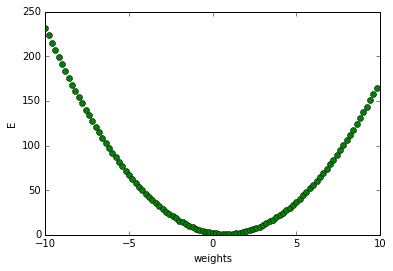
\includegraphics[width=0.5\textwidth]{EFunction}
\end{figure}

\begin{figure}[h]
  \centering
  \caption{$\varepsilon(w)$ (green circles) and a weight path (blue diamonds connected with a line), $\eta = 0.1$. Minimum weight = 0.750126949946, number of iteration = 18 \label{fig:EFunction01}}
  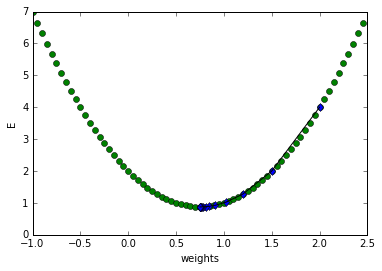
\includegraphics[width=0.5\textwidth]{EFunction01}
\end{figure}

\begin{figure}[h]
  \centering
  \caption{$\varepsilon(w)$ (green circles) and a weight path (blue diamonds connected with a line), $\eta = 0.01$. Minimum weight = 0.752326375959, number of iteration = 154 \label{fig:EFunction001}}
  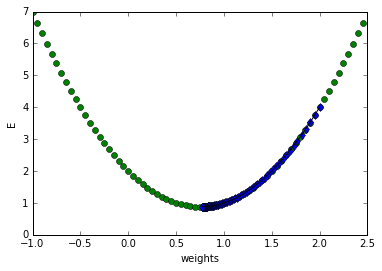
\includegraphics[width=0.5\textwidth]{EFunction001}
\end{figure}

\begin{figure}[h]
  \centering
  \caption{$\varepsilon(w)$ (green circles) and a weight path (blue diamonds connected with a line), $\eta = 0.45$. Minimum weight = 0.750043556143, number of iteration = 46  \label{fig:EFunction045}}
  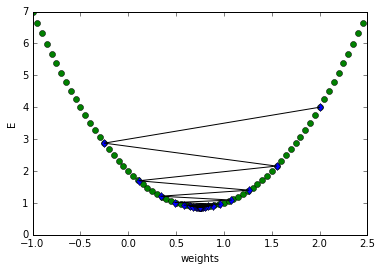
\includegraphics[width=0.5\textwidth]{EFunction045}
\end{figure}

As we can see, the smoothest trajectory is with the smallest $\eta$ - the transient response is overdamped, it converges quite slow. Large $\eta$ shows zigzag behavior and if we continue to increase the $\eta$, the oscillations and a number of iterations will increase (see Fig.\ref{fig:EFunction049}). Finally, if we try to plot the path with $\eta \geqslant 0.5$ the algorithms diverges.

\begin{figure}[h]
  \centering
  \caption{$\varepsilon(w)$ (green circles) and a weight path (blue diamonds connected with a line), $\eta = 0.49$. Minimum weight = 0.749951866545, number of iteration = 249  \label{fig:EFunction049}}
  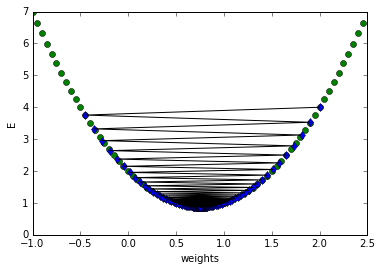
\includegraphics[width=0.5\textwidth]{EFunction049}
\end{figure}

So, small $\eta$s give a better result, but they might require too many iterations and one should be careful with large $\eta$s because they can start oscillate.\\

\cleardoublepage	

\subsection{Exercise 3.2}

Consider the cost function\\
$\varepsilon(\boldsymbol{w}) = \frac{1}{2} \sigma^2 - \boldsymbol{\boldsymbol{r}}_{xd}^T\boldsymbol{w} + \frac{1}{2}\boldsymbol{w}^T\boldsymbol{R}_x\boldsymbol{w}$,\\

where $\sigma^2$ is a constant and

\[\boldsymbol{r}_{\boldsymbol{x}d} = \left( \begin{array}{ccc}
0.8182 \\
0.354 \end{array} \right)\]

\[\boldsymbol{R}_x = \left( \begin{array}{ccc}
1 & 0.8182 \\
0.8182  & 1 \end{array} \right)\]

(a) Find the optimum value $\boldsymbol{w}*$ for which $\varepsilon(\boldsymbol{w})$ reaches its minimum value.

(b) Use the method of steepest descent to compute $\boldsymbol{w}*$ for the following two values of learning-rate parameter: $\eta = 0.3$, $\eta = 1.0$. For each case, plot the trajectory by evolution of the weight vector $\boldsymbol{w}(n)$ in the W-plane.\\

Solution:\\


\subsection{Exercise 3.4}
The correlation matrix $R_x$ of the input vector $x(n)$ in the LMS algorithm is defined by

\[ R_x = \left( \begin{array}{ccc}
1 & 0.5 \\
0.5  & 1 \end{array} \right)\]

Define the range of values for the learning-rate parameter $\eta$ of the LMS algorithm for it to be convergent in the mean square.\\

Solution:\\

The algorithm converges if:\\

$0 < \eta < \frac{2}{\lambda_{max}}$,\\
where $\lambda_{max}$ is the larges eigenvalue of the correlation matrix $R_x$.\\

 \[ R_x - \lambda I = \left| \begin{array}{ccc}
1 - \lambda & 0.5 \\
0.5 & 1 - \lambda \end{array} \right| = \lambda^2 - 2\lambda + 0.75,\]
so $\lambda_1 = 1.5$ and $\lambda_2 = 0.5$. Therefore, $\lambda_{max} = 1.5$ and:

$0 < \eta < \frac{2}{1.5} \Rightarrow 0 < \eta < 1.3333$

\smallskip
Countour plots for error function and descent trajectory for different $\eta$.

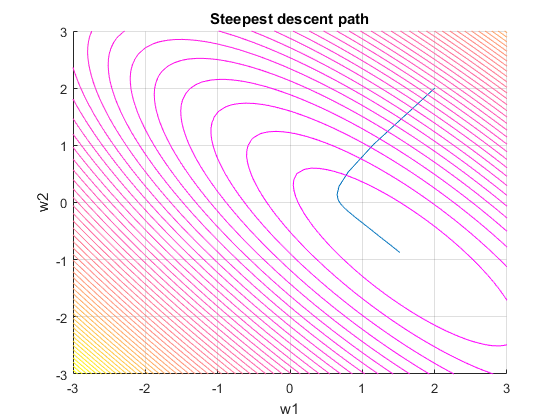
\includegraphics[scale = 1]{d1.png}

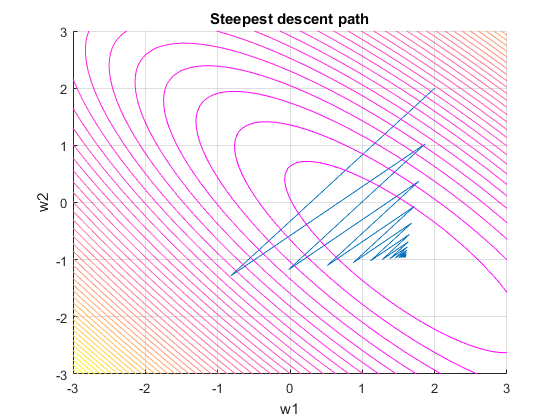
\includegraphics[scale = 1]{d2.png}

\smallskip

Optimal weight vector: $w* = [ 1.4779,-0.8332]$.


\newpage

Matlab code for steepest descent:
\medskip
\lstinputlisting{Ex32.m}

\subsection{Exercise 3.8}
The ensemble-averaged counterpart to the sum of error squares viewed as a cost function is the mean-square value
of the error signal:

\begin{equation*}
J(w) = \frac{1}{2}E[e^2(n)] = \frac{1}{2}E[(d(n) - \mathbf{x}^T(n)\mathbf{w})^2]
\end{equation*}

Assuming that the input vector $x(n)$ and desired response $d(n)$ are drawn from a stationary environment, show that:


\subsection*{Assignment a)}
Assuming that the input vector $x(n)$ and desired response $d(n)$ are drawn from a stationary environment, show that
    \begin{equation*}
        J(w) = \frac{1}{2}\sigma^2_d\mathbf{r_x}_d^T\mathbf{w}+
        \frac{1}{2}\mathbf{w}^T\mathbf{R_x}\mathbf{w}
    \end{equation*}
    where

    \begin{equation*}
        \sigma_d^2 = E[d^2(n)]
    \end{equation*}


    \begin{equation*}
        \mathbf{r_x}_d = E[\mathbf{x}(n)d(n)]
    \end{equation*}

    \begin{equation*}
        \mathbf{R_x} = E[\mathbf{x}(n)\mathbf{x}^T(n)]
    \end{equation*}
\subsection*{Solution a)}


$$
\begin{array}{l}
J(w) = \frac{1}{2}E[(d(n) - \mathbf{x}^T(n)\mathbf{w})^2] = \frac{1}{2}E[d(n)^2 - 2 d(n)\mathbf{x}^T(n)\mathbf{w}+\mathbf{x}^T(n)\mathbf{w}\mathbf{x}^T(n)\mathbf{w}] = \\
\\
=\frac{1}{2}(E[d(n)^2] - 2E[\mathbf{x}(n)d(n)]\mathbf{w}+E[\mathbf{w}^T\mathbf{x}(n)\mathbf{x}(n)^T\mathbf{w}]) =\\
\\
=\frac{1}{2}\sigma_d^2 - \mathbf{r_x}_d^T\mathbf{w} + \mathbf{w}^T E[\mathbf{x}(n)\mathbf{x}(n)^T] \mathbf{w} = \frac{1}{2}\sigma_d^2 - \mathbf{r_x}_d^T\mathbf{w} +\frac{1}{2}\mathbf{w}^T \mathbf{R_x} \mathbf{w} = J(w).
\end{array}
$$

\subsection*{Assignment b)}
For this cost function, show that the gradient vector and Hessian matrix of $J(w)$ are as follows, respectively:
$$
\begin{array}{l}
   g = - \mathbf{r_x}_d +\mathbf{R_x}\mathbf{w}\\
   \mathbf{H} = \mathbf{R_x}
\end{array}
$$

\subsection*{Solution b)}
Gradient vector:
\begin{equation*}
  \mathbf{g}= \frac{\partial J}{\partial w} = \frac{\partial (\frac{1}{2}\sigma_d^2 - \mathbf{r_x}_d^T\mathbf{w} +\frac{1}{2}\mathbf{w}^T \mathbf{R_x} \mathbf{w})}{\partial w} = 0-\mathbf{r_x}_d+\mathbf{R_x} \mathbf{w} =-\mathbf{r_x}_d+\mathbf{R_x} \mathbf{w} .
\end{equation*}
Hessian matrix:

\begin{equation*}
  \mathbf{H}= \frac{\partial \mathbf{g}}{\partial w} = \frac{\partial (-\mathbf{r_x}_d^T+\mathbf{R_x} \mathbf{w})}{\partial w} = \mathbf{R_x}.
\end{equation*}

\subsection*{Assignment c)}

In the LMS/Newton algorithm, the gradient vector $g$ is replaced by its instantaneous value (Widrow and
Strearns,1985).Show that this algorithm, incorporating a learning-rate parameter $\eta$, is described by
\begin{equation*}
  \mathbf{\hat{w}}(n+1)= \mathbf{\hat{w}}(n)+\eta \mathbf{R_x}^{-1} \mathbf{x}(n)(d(n) - \mathbf{x}^T(n) \mathbf{w}(n) ).
\end{equation*}

The inverse of the correlation matrix $\mathbf{R_x}$, assumed to be positive definite, is calculated ahead of time.
\subsection*{Solution c)}
In the Newton's method we have the following rule:
\begin{equation*}
  w_{k+1} = w_{k} - \eta \mathbf{R}^{-1}\mathbf{g},
\end{equation*}
replace $g$ with instantaneous values by omitting Expectations:
\begin{equation*}
  \hat{g} = - \mathbf{r_x}_d +\mathbf{R_x}\mathbf{w} = -\mathbf{x}(n)d(n) + \mathbf{x}(n)\mathbf{x}^T(n)\mathbf{w}(n).
\end{equation*}
So, LMS/Newton algorithm will be:
$$
\begin{array}{l}
  \hat{w}_{k+1} = \hat{w}_{k} - \eta \mathbf{R}^{-1}\hat{g} =\\
  \\
  =\hat{w}_{k} - \eta \mathbf{R}^{-1}(-\mathbf{x}(n)d(n) + \mathbf{x}(n)\mathbf{x}^T(n)\mathbf{w}(n)) =\\
  \\
  =\mathbf{\hat{w}}(n)+\eta \mathbf{R_x}^{-1} \mathbf{x}(n)(d(n) - \mathbf{x}^T(n) \mathbf{w}(n) ).
\end{array}
$$
\end{document}
